\begin{enumerate}[label=\thesection.\arabic*.,ref=\thesection.\theenumi]
\numberwithin{equation}{enumi}

\item The open loop transfer function of a system is 
\begin{align}
G(s) = \frac{2}{(s+1)(s+2)}
\label{eq:ee18btech11017_system}
\end{align}
Find its magnitude and phase response.
\\
\solution Substituting $s = \j\omega$ in \eqref{eq:ee18btech11017_system},

\begin{align}
G\brak{\j\omega}&=\frac{1}{\brak{j\omega+1}\brak{j\omega+2}} 
\\
\implies 
\abs{G\brak{\j\omega}}&=\frac{2}{\brak{\sqrt{\omega^2+1}}\brak{\sqrt{\omega^2+4}}}
\label{eq:ee18btech11017_gain}
\\
\angle G\brak{\j\omega}&=- \tan^{-1}(\omega) - \tan^{-1}\brak{\frac{\omega}{2}} 
\label{eq:ee18btech11017_phase}
\end{align}

\item Find $\omega$ for which the gain of \eqref{eq:ee18btech11017_system} first becomes 1.
\\
\solution From \eqref{eq:ee18btech11017_gain}

\begin{align}
\abs{G\brak{\j\omega}}&=1
\\
\implies \frac{2}{\brak{\sqrt{\omega^2+1}}\brak{\sqrt{\omega^2+4}}}&=1
\\
\implies \omega_{gc}&=0
\end{align}
which is the desired frequency.

\item Find $\angle G(\j\omega_{gc}) + 180\degree$.  This is known as the {\em phase margin}(PM)
\\
\solution From \eqref{eq:ee18btech11017_phase},
%
\begin{align}
\angle G\brak{\j\omega} = 0\degree
\implies PM=180\degree
\label{eq:ee18btech11017_pm}
\end{align}
%
\item Verify your result by plotting the gain and phase plots of $G(\j\omega)$.
\\
\solution The following code plots Fig. \ref{fig:ee18btech11017}

\begin{lstlisting}
codes/ee18btech11017.py
\end{lstlisting}
%
The Phase plot is as shown,
\begin{figure}[!h]
  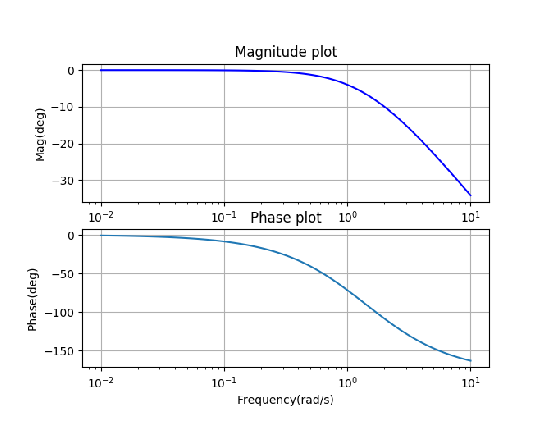
\includegraphics[width=\columnwidth]{./figs/ee18btech11017.eps}
  \caption{}
  \label{fig:ee18btech11017}
\end{figure}

\item A positive phase margin for the open loop system indicates a stable closed loop system.  \eqref{eq:ee18btech11017_pm} indicates that $G(s)$ with unity feedback is stable.  Show that the roots of $1+G(s)$ lie in the left half plane proving closed loop stability.
\\
\solution  Let the closed loop transfer function
\begin{align}
T(s)=\frac{G(s)}{1+G(s)}
\end{align}
Then
\begin{align}
1+G(s)&=0 
\\
\implies s^{2}+3s+4&=0 
\\
\text{or } s&=-1.5+1.3j,-1.5-1.3j
\end{align}
Since the roots are in the left half plane, the system is stable.
%

\item Instead of unity feedback, consider a system with 
%
\begin{align}
H(s)=\frac{50}{s+1}
\end{align}
%
Compute the open loop phase margin for this system.
\\
\solution 
%
\begin{align}
\because G(s)H(s)=\frac{100}{(s+1)^{2}(s+2)},
\label{eq:ee18btech11017_gh}
\end{align}
%
the  magnitude and phase are
\begin{align}
\label{eq:ee18btech11017_gh_mag}
\abs{G\brak{\j\omega}H\brak{\j\omega}}&=\frac{10^{2}}{ \sqrt{(\omega^{2}+1)^{2}}
\sqrt{\omega^{2}+4}} \\
\angle G\brak{\j\omega}H\brak{\j\omega}&=-\tan^{-1}\frac{\omega}{2}-2\tan^{-1}(\omega) 
\label{eq:ee18btech11017_gh_ang}
\end{align}
%
The gain crossover frequency is given by 
\begin{align}
\frac{10^{2}}{\sqrt{\omega_{gc}^{2}+4} \sqrt{(\omega_{gc}^{2}+1^{2})^{2}}}&=1 \\
\\
\omega_{gc}^{6}+6\omega_{gc}^{4}+9\omega_{gc}^{2}-9996&=0 
\\
\implies \omega_{gc} &= 4.42  
\label{eq:ee18btech11017_gh_wgc}
\end{align}
%
From \eqref{eq:ee18btech11017_gh_ang} and \eqref{eq:ee18btech11017_gh_wgc},
the phase margin is
\begin{align}
PM &=180\degree-2\tan^{-1}(\omega_{gc})-\tan^{-1}\brak{\frac{\omega_{gc}}{2}} \\
\implies  P.M &=-40.15\degree
\label{eq:ee18btech11017_gh_pm}
\end{align}
\item Verify your result through the magnitude and phase plot.
\\
\solution The following code plots Fig. \ref{fig:ee18btech11017_2}
\begin{lstlisting}
codes/ee18btech11017_2.py
\end{lstlisting}
\begin{figure}[!h]
  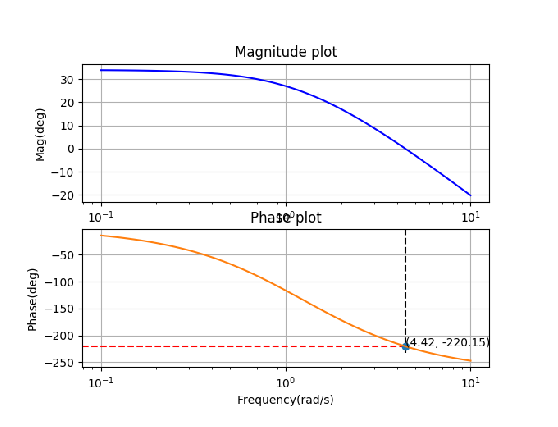
\includegraphics[width=\columnwidth]{./figs/ee18btech11017_2.eps}
 \caption{}
  \label{fig:ee18btech11017_2}
\end{figure}
%
\item Since the PM in \eqref{eq:ee18btech11017_gh_pm} is negative, the closed loop system is unstable .
Verify this using the Routh-Hurwitz criterion.
%
\\
\solution 
The characteristic equation is 
\begin{align}
1+G(s)H(s)&=0 
\\
\implies s^{3}+4s^{2}+5s+102=0   
\label{eq:ee18btech11017_gh_char}
\end{align}
Constructing the routh array for \eqref{eq:ee18btech11017_gh_char},

\begin{align}
\mydet{s^3\\s^2\\s}
\mydet{1 & 5 & 0 \\ 4 & 102 & 0 \\ -20.5 & 0 & 0}
\\
\mydet{s^3\\s^2\\s\\s^0}
\mydet{1 & 5 & 0 \\ 4 & 102 & 0 \\ -20.5 & 0 & 0 \\ 102 & 0 & 0}
\end{align}

$\because $ there are two sign changes in the first column of the routh array,  two  poles lie on right half of s-plane.  Therefore,the system is unstable.


\end{enumerate}
